\documentclass[crop=false, class=memoir]{standalone}
\usepackage[utf8]{inputenc}%Nødvendig for danske bogstaver
\usepackage[danish]{babel}%Sørger for at ting LaTeX gør automatisk er på dansk
\usepackage{csquotes}
\usepackage{geometry}%Til opsætning af siden
\geometry{lmargin = 2.5cm,rmargin = 2.5cm}%sætter begge magner
\usepackage{lipsum}%Fyldtekst, til brug under test af layoutet
\usepackage{float}
\usepackage{graphicx}%Tillader grafik
\usepackage{epstopdf}%Tillader eps filer
\usepackage{marginnote}% Noter i margen
\interfootnotelinepenalty=10000 %undgår at fodnoter bliver spilittet op.
\usepackage[sorting=none]{biblatex}
\addbibresource{litteratur.bib}
\usepackage[hidelinks]{hyperref}%Tillader links
\usepackage{subcaption} % Tillader underfigurer
\usepackage[font={small,sl}]{caption}	% Caption med skrå tekst ikke kursiv

\usepackage{xcolor} %Bruges til farver
\usepackage{forloop} %Bruges til nemmere for loops

\newcounter{opgave}[chapter] %Definerer opgavenumrene og hvornår de nulstilles
\renewcommand{\theopgave}{\thechapter.\arabic{opgave}} %Definerer udseende af opgavenummereringen
\newcounter{delopgave}[opgave] %Definerer delopgavenumrene
\newcounter{lvl} %Definerer en "variabel" til senere brug

\definecolor{markerColor}{rgb}{0.0745098039, 0.262745098, 0.584313725} %Definerer farven af markøren
\newcommand{\markerSymbol}{\ensuremath{\bullet}} %Definerer tegnet for markøren
\newlength{\markerLength} %Definerer en ny længde
\settowidth{\markerLength}{\markerSymbol} %Sætter den nye længde til bredden af markøren

\newenvironment{opgave}[2][0]{%Definerer det nye enviroment, hvor sværhedsgraden er den første parameter med en default på 0
\newcommand{\opg}{\refstepcounter{delopgave}\par\vspace{0.1cm}\noindent\textbf{\thedelopgave)\space}}%Definerer kommando til delopgave
\refstepcounter{opgave}%Forøger opgavenummer med 1 og gør den mulig at referere til
\setcounter{lvl}{#1}%Sætter "variablen" lvl lig med angivelsen af sværhedsgraden
\noindent\hspace*{-0.75em}\hspace*{-\value{lvl}\markerLength}\forloop{lvl}{0}{\value{lvl}<#1}{{\color{markerColor}\markerSymbol}}\hspace*{0.75em}%Sætter et antal af markører svarende til sværhedsgraden
\textbf{Opgave \theopgave : #2}\newline\nopagebreak\ignorespaces}{\bigskip} %Angiver udseende af titlen på opgaverne samt mellemrummet mellem opgaver



\usepackage{mathtools}%Værktøjer til at skrive ligninger
\renewcommand{\phi}{\varphi}%Vi bruger varphi
\renewcommand{\epsilon}{\varepsilon}%Vi bruger varepsilon
\usepackage{physics}%En samling matematikmakroer til brug i fysiske ligninger
\usepackage{braket}%Simplere kommandoer til bra-ket-notation
\usepackage{siunitx}%Pakke der håndterer SI enheder godt
\DeclareSIUnit\clight{\text{\ensuremath{c}}} % Lysets fart i vakuum som c og ikke c_0
\usepackage{chemmacros}
\usechemmodule{isotopes}
\usepackage{tikz}
\usepackage[danish]{cleveref}
\usepackage{nicefrac}
% \renewcommand{\ref}[1]{\cref{#1}}
\creflabelformat{equation}{#2(#1)#3}
\crefrangelabelformat{equation}{#3(#1)#4 to #5(#2)#6}
\crefname{equation}{ligning}{ligningerne}
\Crefname{equation}{Ligning}{Ligningerne}
\crefname{section}{afsnit}{afsnitene}
\Crefname{section}{Afsnit}{Afsnitene}
\crefname{figure}{figur}{figurene}
\Crefname{figure}{Figur}{Figurene}
\crefname{table}{tabel}{tabellerne}
\Crefname{table}{Tabel}{Tabellerne}
\crefname{opgave}{opgave}{opgaverne}
\Crefname{opgave}{Opgave}{Opgaverne}
\crefname{delopgave}{delopgave}{delopgaverne}
\Crefname{delopgave}{Delopgave}{Delopgaverne}

\newcommand{\eqbox}[1]{\begin{empheq}[box=\fbox]{align}
	\begin{split}
	#1
	\end{split}
\end{empheq}}

\newcommand{\kb}{\ensuremath{k_\textsc{b}}}

\DeclareSIUnit{\parsec}{pc}
\DeclareSIUnit{\lightyear}{ly}
\DeclareSIUnit{\astronomicalunit}{AU}
\DeclareSIUnit{\year}{yr}
\DeclareSIUnit{\solarmass}{M_\odot}
\DeclareSIUnit{\solarradius}{R_\odot}
\DeclareSIUnit{\solarluminosity}{L_\odot}
\DeclareSIUnit{\solartemperature}{T_\odot}
\DeclareSIUnit{\earthmass}{M_\oplus}
\DeclareSIUnit{\earthradius}{R_\oplus}
\DeclareSIUnit{\jupitermass}{M_J}

% Infobokse og lignende
% http://mirrors.dotsrc.org/ctan/graphics/awesomebox/awesomebox.pdf
% \usepackage{awesomebox}


% Egen infobokse (virker kun med begrænsede symboler)

\usepackage[framemethod=tikz]{mdframed}
\usetikzlibrary{calc}
\usepackage{kantlipsum}

\usepackage[tikz]{bclogo}

\tikzset{
    % lampsymbol/.style={scale=2,overlay}
    % lampsymbol/.pic={\centering\tikz[scale=5]\node[scale=10,rotate=30]{\bclampe}}.style={scale=2,overlay}
    infosymbol/.style={scale=2,overlay}
}

\newmdenv[
    hidealllines=true,
    nobreak,
    middlelinewidth=.8pt,
    backgroundcolor=blue!10,
    frametitlefont=\bfseries,
    leftmargin=.3cm, rightmargin=.3cm, innerleftmargin=2cm,
    roundcorner=5pt,
    % skipabove=\topsep,skipbelow=\topsep,
    singleextra={\path let \p1=(P), \p2=(O) in ($(\x2,0)+0.92*(1.1,\y1)$) node[infosymbol] {\bcinfo};},
    % singleextra={\path let \p1=(P), \p2=(O) in ($(\x2,0)+0.5*(2,\y1)$) node[infosymbol] {\bcinfo};},
]{info}

% Skal bruges som
% \begin{info}[frametitle={Titel}]
%     Tekst
% \end{info}

\begin{document}
\chapter{Kosmologi} \label{chap:kosmo_facit}

\begin{opgave}{Hubbleloven}
    \opg Hubbleloven beskriver universets udvidelse, der får alting til at bevæge sig væk fra hinanden. Negative hastigheder betyder, at himmellegemer bevæger sig imod os, hvilket ikke kan skyldes universets udvidelse. Ergo gælder Hubbleloven kun for objekter med $v > 0$. Hvis man prøvede alligevel, ville man få en negativ længde, og det giver ikke mening.
    \opg Lys bliver blåforskudt, når lyskilden bevæger sig imod modtageren. Af spørgsmål \textbf{1}) gælder Hubbleloven derfor ikke.
\end{opgave}

\begin{opgave}{Den kritiske tæthed}
\opg Hvis universet er fladt, har det ingen krumning, hvorfor $\kappa = 0$.
\opg Indsættes $\kappa = 0$ i Friedmannligningen fås
%
\begin{align*}
    H^2 &= \frac{8\pi G \rho}{3} + \frac{\Lambda}{3}, \\
    \implies H^2 - \frac{\Lambda}{3} &= \frac{8\pi G}{3}\rho.
\end{align*}
%
Ganges brøken over fås
%
\begin{align*}
    \rho_c = \frac{1}{8\pi G}\left(3H^2 - \Lambda\right).
\end{align*}
%
\opg $\Lambda \ll 3H^2 \implies 3H^2 - \Lambda \simeq 3H^2$ hvorfor
%
\begin{align*}
    \rho_c \simeq \frac{3H_0^2}{8\pi G}.
\end{align*}
%
\opg Bruges værdierne $H_0 = \SI{70}{\kilo\metre\per\second\per\mega\parsec}$ og $G = \SI{6,6742e-11}{\newton\metre\squared\per\kilo\gram\squared}$ fås
%
\begin{align*}
    \rho_\text{c} \simeq \frac{3H_0^2}{8\pi G} = \frac{3(\SI{70}{\kilo\metre\per\second\per\mega\parsec})^2}{8\pi\cdot\SI{6,6742e-11}{\newton\square\metre\per\square\kilo\gram}} =  \SI{9.2e-27}{\kilo\gram\per\cubic\metre}.
\end{align*}
\end{opgave}



\begin{opgave}{Dopplerforskydning}
	\opg 
	\begin{figure}[h!]
		\centering
		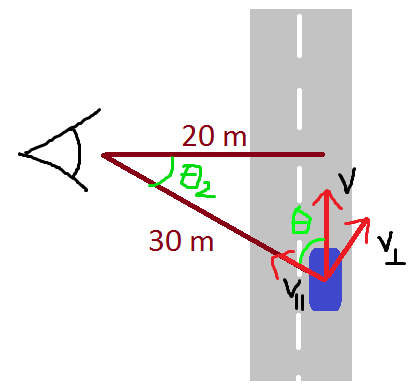
\includegraphics[width=0.5\textwidth]{Kosmo/kosmofig/PolitiLoesning.png}
		%\caption{Et typisk } %https://upload.wikimedia.org/wikipedia/commons/9/98/Andromeda_Galaxy_%28with_h-alpha%29.jpg
	\end{figure}
	\opg Den radielle hastighed er den parallele komponent med synsvinklen. Vi ser en retvinklet trekant og bruger
	\begin{align}
		\cos(\theta)=\frac{\text{hosliggende katete}}{\text{hypotenusen}}=\frac{v_\textup{radiel}}{v} \\
		v_\textup{radiel}=v \cos(\theta)
	\end{align}
	Der dannes også en retvinklet trekant af vejen, afstanden til vejen og afstanden til bilen. I grader giver det en vinkel på
	\begin{align}
		\cos(\theta_2)&=\frac{20}{30}\\
		\theta_2 &= \cos^{-1} \left( \frac{20}{30} \right) = 48
	\end{align}
	De to vinkler indgår begge i en retvinklet trekant, så
	\begin{align}
		180 &= \theta + \theta_2 + 90\\
		\theta &= 90 - \theta_2  = 42
	\end{align}
	Vi indsætter og får
	\begin{align}
	v_\textup{radiel} = \SI{50}{\kilo\meter\per\hour} \cdot \cos(42) = \SI{50}{\kilo\meter\per\hour} \cdot \num{0.74} = \SI{37}{\kilo\meter\per\hour}
	\end{align}
	Hvis du ikke får det samme, så prøv at regne alt i radianer, da det er simplere.
	\opg 
	Du står stille, så $v_\textup{kilde} = \SI{0}{\meter\per\second}$. $v_\textup{obs}$ er den radielle hastighed, som lige skal omregnes til \si{\kilo\meter\per\hour}:
	\begin{align}
	\SI{37}{\kilo\meter\per\hour} = 37 \frac{\SI{e3}{\meter}}{\SI{1}{\hour} \cdot \SI{60}{\minute\per\hour} \cdot \SI{60}{\second\per\minute}} = \frac{37}{\num{3.6}} \si{\meter\per\second} \approx \SI{10.3}{\meter\per\second}
	\end{align}
	Så indsætter vi i
	\begin{align}
	f_\textup{obs} = \frac{\SI{340}{\meter\per\second} + \SI{10.3}{\meter\per\second}}{\SI{340}{\meter\per\second} + \SI{0}{\meter\per\second}} \SI{800}{\hertz} \approx \SI{824}{\hertz}
	\end{align}
    (Hz er enheden hertz, som er 1/s)
\end{opgave}

\begin{opgave}{Skalafaktor}
	Vi ved temperaturen dengang var $T(t) = \SI{3000}{\kelvin}$, og nu er den $T_0 = \SI{2.73}{\kelvin}$. Så vi kan brugem at skalafaktoren ændrer sig med rødforskydningen, og sammensætte det med hvordan den ændrer sig med temperatur:
	\begin{align}
	    a(t) = \frac{1}{1+z} = \frac{T_0}{T(t)}\\
	    z = \frac{T(t)}{T_0} - 1
	\end{align}{}
	Så vi kan nu regne fra temperatur til rødforskydning:
	\begin{align}
	    z = \frac{T(t)}{T_0} - 1 = \frac{\SI{3000}{\kelvin}}{\SI{2.73}{\kelvin}} - 1= \num{1.10e3} - 1 \approx \num{1.10e3}
	\end{align}
	Så der blev dannet atomer ved $z \approx 1100$, da det blev koldt nok til, at elektroner kunne binde sig til atomkernerne.
\end{opgave}

\begin{opgave}{Rødforskydning af kvasar}
	\opg Enheder: $\SI{1}{\angstrom} = \SI{10}{\nano\meter} = \SI{e10}{\meter}$. H-$\alpha$-linjen er ved ca. $\SI{6560}{\angstrom}$. På figuren er det ved omkring $\SI{7600}{\angstrom}$, dvs. bølgelængden er blevet større, så lyset er rødforskudt. Altså må kvasaren bevæge sig væk fra os.\\
	\opg Den radielle hastighed er beskrevet af rødforskydningen. Rødforskydningen er
	\begin{align}
		\frac{\lambda_\textup{obs}-\lambda_\textup{lab}}{\lambda_\textup{lab}} = \frac{\SI{7600}{\angstrom} - \SI{6560}{\angstrom}}{\SI{6560}{\angstrom}} = \num{0,159}.
	\end{align}
	Det er lavt, så vi approksimerer hastigheden til
	\begin{align}
		v= z\cdot c = \num{0,159} \cdot \SI{3e8}{\meter\per\second} = \SI{4,7e7}{\meter\per\second}
	\end{align}
	Regner du det præcist, giver det nogenlunde det samme.
	\opg $\Delta\lambda \approx \SI{200}{\angstrom}$, så det giver $v = \num{0.015} c \approx \SI{4,5e6}{\meter\per\second}$.
\end{opgave}
\begin{opgave}{Afstande}
	\opg Isolér $d_M$ i hvert udtryk.
	\begin{align}
		d_M &= \frac{d_L}{1+z}\\
		d_M &= d_A(1+z)
	\end{align}
	Resultaterne sættes lig hinanden
		\begin{align}
		\frac{d_L}{1+z} &= d_A(1+z)\\
		d_L &= d_A (1+z)^2
		\end{align}
	\opg Ved $z = 1$ er $d_C \approx \SI{3200}{\mega\parsec}$ og derfor
	\begin{align}
		d_L &= d_M (1+z)= \SI{3200}{\mega\parsec} \cdot 2 = \SI{6400}{\mega\parsec}\\
		d_A &= \frac{d_M}{1+z}= \frac{\SI{3200}{\mega\parsec}}{2} = \SI{1600}{\mega\parsec}.
	\end{align}
	Ved $z = 9$ er $d_C \approx \SI{9200}{\mega\parsec}$, så
	\begin{align}
		d_L &= d_M(1+z)= \SI{9200}{\mega\parsec} \cdot 10 = \SI{92000}{\mega\parsec}\\
		d_A &= \frac{d_M}{1+z}= \frac{\SI{9200}{\mega\parsec}}{10} = \SI{920}{\mega\parsec}.
	\end{align}
	Gamle objekter, der har bevæget sig fra os længere tid, har altså en større luminositetsafstand, men en lavere vinkelafstand ved høje rødforskydninger. Man skulle ellers tro objekter så mindre ud på himlen, jo længere væk de var, hvilket er rigtigt indtil omkring $z = \num{1,6}$. I det tidlige univers var galakserne tættere på hinanden, så de fyldte meget på himlen for hinanden, og derfor er deres lys spredt ud over et stort område.
	\opg
	%Dengang var universet for resten kun 250 mio. år gammelt.\\
	Hvis vi approksimerer $z \approx \frac{v}{c}$, får vi overlyshastigheder, så det går ikke.
	\begin{align}
    	z+1 &= \sqrt{\frac{1+\frac{v}{c}}{1-\frac{v}{c}}}\\
    	(z+1)^2 &= \frac{1+\frac{v}{c}}{1-\frac{v}{c}}
	\end{align}
	så vi skal løse et system på formen $y = \frac{1+x}{1-x}$, hvor $y = (z+1)^2$ og $x = \frac{v}{c}$. Man kan omformulere det til $x = \frac{y-1}{y+1}$, ved
	\begin{align}
	    1+x &= y(1-x)\\
	    1+x &= y-yx \\
	    x+yx &= y-1 \\
	    x(1+y) &= y-1 \\
	    x &= \frac{y-1}{y+1}.
	\end{align}
    Derfor må
	\begin{align}
    	\frac{v}{c}&=\frac{(z+1)^2-1}{(z+1)^2+1}\\
    	v&=\frac{(z+1)^2-1}{(z+1)^2+1} c = \frac{(10+1)^2-1}{(10+1)^2+1} c = \num{0.98} c. %3\cdot 10^{8} m/s =
	\end{align}
	Så svaret er \SI{98}{\percent} af lysets fart i vakuum.
\end{opgave}

\begin{opgave}{Andromeda-galaksen}
	\opg 
	\begin{align}
		D_H = \frac{v}{H_0} 
	\end{align}
	Vi skal bruge den radielle hastighed
	\begin{align}
		v \approx z c = \num{-0.001} \cdot \SI{3e8}{\meter\per\second} = \SI{-3e5}{\meter\per\second}
	\end{align}
	og omskriver Hubble-konstanten en lille smule
	\begin{align}
		H_0 = \SI{70}{\kilo\meter\per\second\per\mega\parsec} = \SI{7e4}{\meter\per\second\per\mega\parsec}.
	\end{align}
	Vi indsætter
	\begin{align}
	D_H = \frac{\SI{-3e5}{\meter\per\second}}{\SI{7e4}{\meter\per\second\per\mega\parsec}} = - 3/7 \cdot \SI{10}{\mega\parsec} \approx \SI{-4.3}{\mega\parsec}.
	\end{align}
	Så Hubble-afstanden bryder sammen og giver noget negativt. Ligesom i den første opgave, kan man ikke bruge Hubbles lov på negative rødforskydninger.
	
	\opg Vi omregner lysår (\si{\lightyear}) til meter, så vi kan dividere med den radielle hastighed i \si{\meter\per\second} fra før og få en tid:
	\begin{align}
		\SI{2.5e6}{\lightyear} \approx \num{2.5e6} \cdot \SI{9.46e15}{\meter} = \SI{23.7e21}{\meter}\\
		\frac{\SI{23.7e21}{\meter}}{\SI{3e5}{\meter\per\second}} = \SI{7.9e16}{\second} = \SI{2.5e9}{\year}
	\end{align} 
	Så det vil tage \SI{2.5e9}{\year}, hvis vi ser bort fra accelerationen og andre effekter.
	Stjernerne ligger meget spredt i begge galakser, så det er ekstremt usandsynligt at vi kommer til at støde ind i andre - men det kan sagtens være solsystemet bliver slynget langt ud eller måske helt væk fra galakserne (så udsigten ændres men derudover betyder det ikke så meget for os). Når gassen fra galakserne kolliderer varmes det op, og vi vil derfor se en masse ny stjernedannelse. Galakserne vil med tiden smelte sammen til en elliptisk galakse, der har opbrugt det meste gas, så stjernedannelsen stopper.
\end{opgave}


\begin{opgave}{Et univers af bolde}
\opg Isoleres $n_\textup{b}$ i ligning \eqref{eq:antalsdensitet} og indsættes værdierne $m_\textup{b} = \SI{1}{\solarmass}$ og $\rho_\textup{c} = \SI{8.6e-27}{\kilo\gram\per\cubic\metre}$ fås
%
\begin{align*}
    n_\textup{b} = \frac{\rho_\textup{c}}{m_\textup{b}} = \frac{\SI{8,6e-27}{\kilo\gram\per\cubic\metre}}{\SI{1}{\solarmass}} = \SI{4,3e-57}{\per\cubic\metre} = \SI{1,3e-07}{\per\cubic\parsec}
\end{align*}
\opg Indsættes ovenstående resultat fås
%
\begin{align*}
    d_\textup{b} = n_\textup{b}^{-1/3} = (\SI{4,3e-57}{\per\cubic\metre})^{-1/3} = \SI{200}{\parsec}.
\end{align*}
%\opg Indsættes værdierne $d_\mathrm{b} = \SI{200}{\parsec}$ og $d_\mathrm{max} = \SI{9.8e9}{\parsec}$ fås %,$H_0 = \SI{70}{\kilo\metre\per\second\per\mega\parsec}$ og $\si{\clight} = \SI{3.00e8}{\metre\per\second}$ fås
%
%\begin{align*}
%    \frac{d_\mathrm{max}}{d_\mathrm{b}} = \frac{ \SI{9.8e9}{\parsec} }{\SI{200}{\parsec}} = \SI{4.9e7}{}.
%\end{align*}

%Den gennemsnitlige afstand mellem boldene er altså cirka $4.9\cdot10^{-7}$ gange mindre end afstanden til det fjerneste objekt.

\opg 

\begin{align}
	d_\textup{MFP} = (A n)^{-1} = (\pi R_\odot^2 n)^{-1} = (\pi (\SI{2,25461e-8}{\parsec})^2 \SI{1,3e-07}{\per\cubic\parsec})^{-1} =  \SI{4.9e21}{\parsec} %\SI{2.5e6}{\parsec} 
\end{align}

Så i gennemsnit vil en lysstråle bevæge sig $\SI{4.9e21}{\parsec}$ før den rammer en bold.

\begin{align}
    \frac{d_\textup{max}}{d_\textup{MFP}} = \frac{\SI{9.8e9}{\parsec} }{\SI{4.9e21}{\parsec}} = \num{2e-12} % 3.9e3
\end{align}

Lyset herfra når altså i gennemsnit meget længere end det længste vi faktisk ser. Antaget at det har tid nok til at nå frem.

\opg 

\begin{align}
	P(d_\textup{max}) = e^{-d_\textup{max}/d_\textup{MFP}} = e^{(\num{-3.9e3})} \approx 1
\end{align}

Det kommer meget tæt på 1. %En tiendedel af længden ville have sandsynligheden:
%
%\begin{align}
%	P(d_{max}/10) = e^{-3.9e2} = 5.7e-171
%\end{align}%

%Så det virker ikke til vi ville kunne se ret langt, og universet består nok ikke kun af stjerner med denne fordeling, størrelse, antagelser om kosmologi m.m. Hvis man kunne se en galakse på afstanden $d_{max}$ i et sådan univers alligevel, så ville retningen være meget speciel og et brud på isotropi.

\opg 

\begin{align}
	P(x) = e^{-x/(\pi R_\odot^2 n)^{-1}} = e^{-x \pi R_\odot^2 n} = e^{-x \pi R_\odot^2 \frac{\rho_\textup{c}}{m_\textup{b}}}
\end{align}
Øget radius mindsker sandsynligheden for at se langt, og ved øget masse stiger den. Det afhænger dog mest af radius. Så fordobles begge vil vi kunne se kortere. Med andre ord vil objekter der fylder meget i forhold til deres masse gøre vi ser kortere. 

%Det kosmologiske princip siger, at universet er homogent og isotropt -- altså at massen er jævnt fordelt over hele universet, og at det ser ens ud i alle retninger. Hvis vi skal kunne se noget i afstanden $d_\mathrm{max}$ i et univers kun bestående af bolde, så skal der være et retning, hvor den nærmeste bold er i den afstand. Skal man kunne se cirka 49 millioner gange længere end den gennemsnitlige afstand mellem bolde, så svarer det løst sagt til at der mangler 49 millioner bolde i en bestemt retning, og de må jo så være et andet sted i universet. Det ville dog betyde at der er forskel på hvilken retning vi kigger i, og at massetætheden ikke er den samme alle steder. Det er derfor usandsynligt, at have et univers bestående af sådanne ens bolde, hvor universet har den nuværende massetæthed, hvor vi kan se noget i afstanden $d_\mathrm{max}$, mens det kosmologiske princip er gældende. Det er ikke direkte i modstrid med det kosmologiske princip, da \SI{2,2e7}{M_\odot} ikke er voldsomt stort på kosmologisk skala -- til sammenligning er massen af mælkevejen $\sim \SI{1e12}{M_\odot}$ -- men det er stort nok til at være betydningsfuldt.
\opg 

\begin{align}
    P(d_\textup{max})  = e^{-d_\textup{max} \pi R_\textup{ballon}^2 \frac{\rho_\textup{c}}{m_\textup{ballon}}} =  e^{-d_\textup{max} \pi (0.2/(\num{3.0857e16}) \si{\parsec})^2 \frac{\rho_\textup{c}}{\SI{0.005}{\kilogram}}} = \num{4e-29}
\end{align}

Det virker altså til utroligt lidt lys ville nå frem til os i et univers af balloner, medmindre vi bryder det kosmologiske princip for at skabe en særligt tyndt populeret bane til lyset. 

Det giver mening når vi har fastlagt en bestemt overordnet densitet af universet $\rho_c$, at hvis vi fordeler massen i objekter med lav densitet, så vil en større del af rummet være fyldt, så der oftere vil være noget i ens synslinje. Reelt er universet altså mere klumpet end balloner er. Vi har tunge strukturer i form af stjerner, galakser og galaksehobe. 

%Hele udregningen byggede på en antagelse om at universet kun består af består af bolde med massen $m_\mathrm{b} = \SI{1}{M_\odot}$. Denne antagelse har svært ved at forklare den afstand vi kan se i universet, hvorfor der må være noget galt med antagelsen. Det mest oplagte er tyngdekraften får masse til at klumpe sig sammen til objekter, der er tungere end 1 solmasse. Dette ses også ved den markante forbedring af $d_\mathrm{max}/d_\mathrm{b}$ ved at bruge Mælkevejens masse. På stor skala er Universet altså bedre beskrevet som en samling af ens galakser end en samling af ens stjerner. Dette viser også at det kosmologiske princip fungerer på store længde skalaer, men ikke på mindre. Det er eksempelvis ikke sandt, at alle dele af Mælkevejen ser ens ud fra Jorden -- der er langt mere masse, hvis vi kigger mod galaksens centrum, end hvis vi kigger i den modsatte retning. Galakser samler sig også i galaksehobe, og bruges massen for sådan en fås, at vi kan se cirka 200 gange længere end den gennemsnitlige afstand mellem bolde i et univers hvor boldene vejer det samme som en galaksehob. Dette tyder på, at universet skal det beskrives på en skala af galakser og galaksehobe. Modellen tager ikke højde for at boldene kan have forskellig masse og derudover er synslængde ikke nok i sig selv til at kunne afgøre om modellen er brugbar. Det virker dog sandsynligt, at Universet på tilpas stor skala opfører sig som en samling af galakser og galaksehobe, da det kosmologiske princip lægger op til, at en model med ens bolde ikke er helt ved siden af.
\end{opgave}

\begin{opgave}[4]{Fra stråling til stof}

\opg Figuren viser en graf af $\rho(t)$ for universets forskellige komponenter - en komponent dominerer i perioden hvor den har højere densitet end alle de andre komponenter.

\opg I én periode har den ene komponent højest densitet, i den næste har en anden komponent højest densitet. For at dette kan lade sig gøre må der være et tidspunkt hvorpå komponenterne har \emph{samme} densitet.

\opg Vi starter med de enhedsløse densiteter, \cref{k-kosmo:eq:densities} (bemærk at vi ignorerer usikkerhederne):
\begin{align}
    \Omega_{\textup{m},0} &= \num{0,31} \\
    \Omega_{\textup{R},0} &= \num{8,24e-5}
\end{align}
Vi vil nu kunne oversætte i mellem enhedsløs densitet og normal densitet, som gøres ved \cref{k-kosmo:eq:omega}:
\begin{align}
    \Omega &= \frac{\rho}{\rho_\textup{c}} \\
    \rho_\textup{c} \cdot \Omega &= \rho
\end{align}
Så finder vi densiteterne
\begin{align}
    \rho_{\textup{m},0} &= \Omega_{\textup{m},0} \cdot \rho_\textup{c} \\
    &= \num{0,31} \cdot \SI{8,6e-27}{\kilogram \per \cubic \metre} \\
    &= \SI{2.67e-27}{\kilogram \per \cubic \metre} \\
    \rho_{\textup{R},0} &= \Omega_{\textup{R},0} \cdot \rho_\textup{c}\\
    &= \num{8,24e-5} \cdot \SI{8,6e-27}{\kilogram \per \cubic \metre} \\
    &= \SI{7.09e-31}{\kilogram \per \cubic \metre}
\end{align}

\opg Når overgangen fra den strålingsdominerede periode til den stofdominerede periode sker, må deres densiteter være ens, som vi fandt frem til tidligere. Vi ønsker at finde rødforskydningen for denne overgang - så vi starter med at bestemme skalafaktoren, da
\begin{align}\label{kosmo_facit:eq:redshift}
    a(t) = \frac{1}{1+z}
\end{align}
For at løse opgaven skal vi altså bestemme den skalafaktor således 
\begin{align}\label{kosmo_facit:eq:dens}
    \rho_\textup{m} = \rho_\textup{R}
\end{align}
Fra kompendiet har vi relation mellem en komponents densitet og skalafaktoren
\begin{align}
    \rho = \rho_0 \cdot a^{-3(1+w)}
\end{align}
Stråling har $w = 1/3$ og stof har $w = 0$. Vi finder derved
\begin{align}
    \rho_{\textup{m}} &= \rho_{\textup{m},0} \cdot a^{-3(1+0)} \\
    &= \rho_{\textup{m},0} \cdot a^{-3} \\
    \rho_{\textup{R}} &= \rho_{\textup{R},0} \cdot a^{-3(1+\frac{1}{3})} \\
    &= \rho_{\textup{R},0} \cdot a^{-3 - \frac{3}{3}} = \rho_{\textup{R},0} \cdot a^{-4}
\end{align}
Disse to sættes nu ind i \cref{kosmo_facit:eq:dens}, og vi løser for $a$
\begin{align}
    \rho_{\textup{m},0}\cdot a^{-3} = \rho_{\textup{R},0} \cdot a^{-4} \\
    \frac{\rho_{\textup{m},0}\cdot a^{-3}}{a^{-4}} = \rho_{\textup{R},0} \\
    \frac{a^{-3}}{a^{-4}} = \frac{\rho_{\textup{R},0}}{\rho_{\textup{m},0}} \\
    a^{-3 + 4} = \frac{\rho_{\textup{R},0}}{\rho_{\textup{m},0}} \\
    a = \frac{\rho_{\textup{R},0}}{\rho_{\textup{m},0}}
\end{align}
Denne skalafaktor kan så indsættes i \cref{kosmo_facit:eq:redshift} for at bestemme rødforskydningen.
\begin{align}
    \frac{\rho_{\textup{R},0}}{\rho_{\textup{m},0}} = \frac{1}{1+z} \\
    (1+z)\cdot \frac{\rho_{\textup{R},0}}{\rho_{\textup{m},0}} = 1\\
    1+z = \frac{1}{\frac{\rho_{\textup{R},0}}{\rho_{\textup{m},0}}} = \frac{\rho_{\textup{m},0}}{\rho_{\textup{R},0}}\\
    z = \frac{\rho_{\textup{m},0}}{\rho_{\textup{R},0}} - 1\\
    z = \frac{\SI{2,67e-27}{\kilogram \per \cubic \metre}}{\SI{7,09e-31}{\kilogram \per \cubic \metre}} -1\\
    z =  \num{0.38e4} - 1 \approx 3800
\end{align}
\end{opgave}

\begin{opgave}[2]{Comahoben}

\opg For hver solluminositet har vi én solmasse. Vi har $\SI{3e13}{\solarluminosity}$, så ergo er
\begin{align}
    M_{\textup{Coma}} &= \SI{3e13}{\solarmass}\\
    &= \num{3e13}\cdot \SI{2e30}{\kilogram} \\
    &= \SI{6e43}{\kilogram}
\end{align}

\opg Vi vil bestemme en masse fra en omdrejningshastighed - til dette bruges \cref{k-kosmo:eq:fart_i_galakse} fra kompendiet, som løses for $M$.
\begin{align}
    v = \sqrt{\frac{GM(R)}{R}}\\
    v^2 = \frac{GM_{\text{Coma}}}{R}\\
    Rv^2 = GM_{\text{Coma}} \\
    M_{\text{Coma}} = \frac{Rv^2}{G}
\end{align}
Vi husker så at konverterer enheder fra lysår til meter ($\SI{1}{\lightyear} = \SI{9,46e15}{\metre}$) og fra kilometer per sekund til meter per sekund.
\begin{align}
    M_{\text{Coma}} &= \frac{\SI{12,5e6}{\lightyear} \cdot \SI{9,46e15}{\metre \per \lightyear} \cdot \left(\num{e3} \cdot \SI{2,38e3}{\metre \per \second}\right)^2}{\SI{6,67e-11}{\newton \square \metre \per \square \kilogram}} \\
    &\updownarrow{\text{Proof by lommeregner}}\\
    &= \SI{1e46}{\kilogram} \\
    &= \SI{5e15}{\solarmass}
\end{align}

\opg Vi snakkede om mørkt stof til forelæsningen - en masse masse (haha) man ikke kan se, men som dog stadig er tilstede i universet. Mørkt stof forklarer den ekstra masse som får galaksen i hobens yderkant til at bevæge sig hurtigere end hvad vi ville forvente baseret på hvor meget hoben lyser.

\end{opgave}

\end{document}